% Document settings
\documentclass[11pt]{article}
% % % % % % % % % % % Define Footer
\usepackage{fancyhdr}
\usepackage[margin=1in]{geometry}
\usepackage[pdftex]{graphicx}
\usepackage{multirow}
\usepackage{setspace}
\usepackage{xcolor}
\pagestyle{plain}
\usepackage[american voltages,oldvoltagedirection]{circuitikz}
%\usepackage[american]{circuitikz}
\usepackage{graphicx}
\usepackage{multirow}
\usepackage{booktabs}
\usepackage{epstopdf}
%\usepackage{MnSymbol,wasysym}
\usepackage{amsmath}
%\usepackage{mathtools}
\usepackage{amssymb}
\usepackage{lipsum}
\usepackage{siunitx}
\setlength\parindent{0pt}
\graphicspath{{images/}{drawings/}}
\usepackage{float}
% % % % % % % % % % % Header footer
% % % % % % % % % % %EDIT THIS % % % % % % % % % % % % % % % % % % % %
\pagestyle{fancy}
\fancyhf{}
\lhead{Tech Memo: Experiment 3-Th\'evenin's Equivalent Circuit}
\rhead{Andrei Tumbar}
\lfoot{EE281}
\cfoot{Date }
\rfoot{Page \thepage}
% % % % % % % % % % % % % % % % % % % % % % % % % % % % % % % % % % % % %

\begin{document}
		\numberwithin{equation}{subsection}
		\numberwithin{figure}{subsection}
	\hspace{6in}
		
\includegraphics[scale=0.9,trim=0cm 0in 0in 0.0in,clip]{RIT_KGCOE1}
\newline

\Huge \textbf{EEEE 281 Experiment 3:\\ Th\'evenin's Equivalent Circuit}\\

\Large
\textbf{From:} Andrei Tumbar [Computer Engineering] \\
\textbf{To: } Section 2 TA: LJ Boone, Harrison Keats \\
\textbf{Date: } Performed: 3/3/20  Due: 3/17/20 \\
\textbf{Subject: } Lab 3-Th\'evenin Equivalent Circuits\\
\textbf{Lab Partner(s): } N/A\\
\vspace{0.5in}
	\begin{table}[h!]
		\centering
		%\caption{Grading Table}
		%\label{Table:Grading Table 1}
		%\begin{tabular}{llllll}
		\begin{tabular}{|l||l|l|l|l|}
			\hline
			Component & Percentage of Grade   & Score \hspace{0.5in} & Comment \hspace{1in}  \\
			\hline
			Report Formatting & 20~\si{\percent} & & \\	 
			\hline
			\hline 
%			Hand Calculations & 10~\si{\percent} &10 &\colorbox{yellow}{All students get credit.} \\	 	 
%			 \hline
			PSPICE: Setup Conditions & 5~\si{\percent} & & \\	 
			 \hline
			PSPICE: Data and Figures & 15~\si{\percent} & & \\	 
			 \hline
			PSPICE: Discussion of Simulation & 15~\si{\percent} & & \\	 
			\hline
			\hline
			Hardware: Experimental Setup & 10~\si{\percent} & & \\	 
			\hline
			Hardware: Experimental Data and Tables & 15~\si{\percent} & & \\	 
			\hline
			Hardware: Discussion of Results & 20~\si{\percent} & & \\	 
			\hline
			\hline
			\textbf{Total Score:}&  & & \\	 
			\hline
			\textbf{Graded By:}&  & & \\	 
			\hline
		\end{tabular}
	\end{table}
\newpage
\section*{Abstract}
%\Large \textbf{Abstract} \\
\normalsize
%The abstract section should contain a summary of what was performed in the lab and should be approximately  200 words.  This should succinctly rephrase the purpose of the laboratory.  It should also refer to the data collected.    \textbf{The abstract should specifically mentioned the Th\'evenin resistance and voltage obtained, as well as the various methods used.}

This laboratory exercise created a complex circuit were a Thevenin voltage and resistance was determined. To determine the equivalent voltage, a break was placed across the load resistor and the voltage was measured. The equivalent resistance was found by removing independent sources and placing a test source. The current through the test source will indicate the equivalent resistance in the Thevenin circuit. The ammeter in the multimeter was used to measure this current while the volt-meter was used to measure the break voltage.

\section {Introduction and Theory}

%Include 1-2 paragraphs that explains the scope of the experiment. Briefly introduce the concept of Th\'evenin's equivalent circuit.  What was the primary purpose of the experiment? If the data collection has deviated in any way from the rest of your section (for example you had to come back to collect more data), explain this in a second paragraph.  In particular, be sure to note if your data was acquired from a different lab than your classmates/using different equipment. 

The scope of this experiment was to find the equivalent Thevenin circuit by measuring the break voltage and the current through a test source. A Thevenin circuit is one consisting of a voltage source and a resistor. According to Thevenin law, this circuit can represent any complex circuit with any configuration of current or voltage sources whether they be dependent or independent.

\subsection{Theory: Circuit Topology}
%In this section, you should introduce the reader to the circuit  investigated in the experiment, and demonstrate the theoretical value of the circuits. 

%\begin{itemize}
%	\item A figure of the circuit schematic should be included here.  You can use a figure from PSPICE. Be sure to indicate what the load resistor is.  Students using \LaTeX  may ask Dr. Rommel permission to use the Circuitikz artwork used in the laboratory handout. Use of the artwork should be appropriately acknowledged as a citation and under the acknowledgements. If you do use Circuitikz, please let Dr. Rommel know what version you are using.  Some recent updates (discovered while writing this handout/tempalte) have changed the way voltage polarity is presented.  You will hae to edit the values of the resistors. 
%	\item Define the ground in the circuit and specific nodes. 
%	\item This description can be short (a few sentences in length).
%\end{itemize}

The circuit in question is one consisting of seven resistors. A list of parameters controls the value of each resistor. Four different variations of the circuit were designed to gain proper measurements in the simulations.

\begin{figure}[h!]
\begin{center}
\begin{circuitikz}

\draw (0,4) to[battery, *-*, l_=$12\,\si\volt$] (0,0)
	  (0,4) coordinate(A)
	  -- ++(0,1.5) to[R, *-*, a^=$R_1$,l_=$5.6\,k\si\ohm$] ++(8,0) coordinate (B)
	  (A) to[R, *-*, a^=$R_2$,l_=$5.6\,k\si\ohm$] ++(4,0)
	  coordinate (C1)
	  
	  to[R, *-*, a^=$R_3$,l_=$5.6\,k\si\ohm$] ++(4,0) coordinate(C)
	  
	  (B) -- (C)
	  to[R, *-*, a^=$R_L$,l_=$5.6\,k\si\ohm$] ++(0,-4)
	  to[R, *-*, a^=$R_5$,l_=$5.6\,k\si\ohm$] ++(-4,0) coordinate(D)
	  to[R, *-*, a^=$R_4$,l_=$5.6\,k\si\ohm$] ++(-4,0)
	  (C1) to[R, *-*, a^=$R_6$,l_=$5.6\,k\si\ohm$] (D)
	  
	  (0,0) node[ground]{}
;

\end{circuitikz}		

\label{fig:circuit}

\end{center}
\end{figure}

Figure \ref{fig:circuit} depicts the circuit in question. All resistors are $5.6\,k\si\ohm$ and the load resistor is labeled $R_L$. A $12\,\si\volt$ power source is connected to power the circuit.

%\subsection{Theory: Hand Calculations and PSPICE of Th\'evenin Equivalent Circuit}
%\colorbox{yellow}{\textcolor{blue}{Hand calculations are \textbf{not} required for this lab report.}}
%
\subsection{Theory: PSPICE Simulation Summary}
%Begin by providing a 1 paragraph description of the PSPICE setup.  Which \textbf{libraries} and \textbf{PSPICE elements} were used in the simulation? You can borrow from the text of your first tech memo here.  If you do so, please be sure to cite the tech memo. Note the libraries used. You can find the information when you look at the properties of each element.  There will be a reference to a ``.olb'' file.  This is the library name. 

The PSPICE simulation began with a design of the circuit. The PSPICE setup used the libraries imported from the Circuits 1 library from the lab computer. The libraries were called \textbf{analog.olb}, \textbf{opamp.olb}, \textbf{source.olb}, and \textbf{special.olb}. The components used were ``R/ANALOG'' from the \textbf{analog.olb} for the resistors, ``VDC/SOURCE'' from the \textbf{source.olb} for the voltage source and ``O/CAPSYM'' and ``PARAMETER/SPECIAL'' from the \textbf{special.olb} for ground.

%Include a description of the resistor sweep.  Specifically, what is the function of the \textbf{PARAMETER/SPECIAL} element?   Also, what type of simluation was run?What were the start/stop resistor values? What was the step size, and was it linearly or logarithmically varied?    Comment about the line fit in Excel (or whatever software was used to perform the linear regression).

A parameter list using the ``PARAMETER/SPECIAL'' component was used to allow the values of each resistor be easily changed. Rcommon controlled the value of every resistor apart from $R_6$ and $R_L$ A resistor sweep was performed in the PSPICE so that the voltage across $R_L$ could be measured for varying values of $R_L$. The slope of the curve would yield the Thevenin resistance while the intercept would represent the Thevenin voltage.

%The lab handout called for using parameters in the tutorial, which were edited during your prelab to match the resistors in this lab.  What changes were made to the parameters?  Also, why were unique names given for Net Aliases in each circuit?
\subsubsection{Theory: PSPICE Schematic Diagram}
%Since the prelab called for having all 4 circuits on the same page, you may place two copies of the schematic here as listed in Figs. \ref{Fig:SchematicVoltMarkers} and \ref{Fig:SchematicCurrentMarkers}

\begin{figure}[h!]
	\begin{center}
		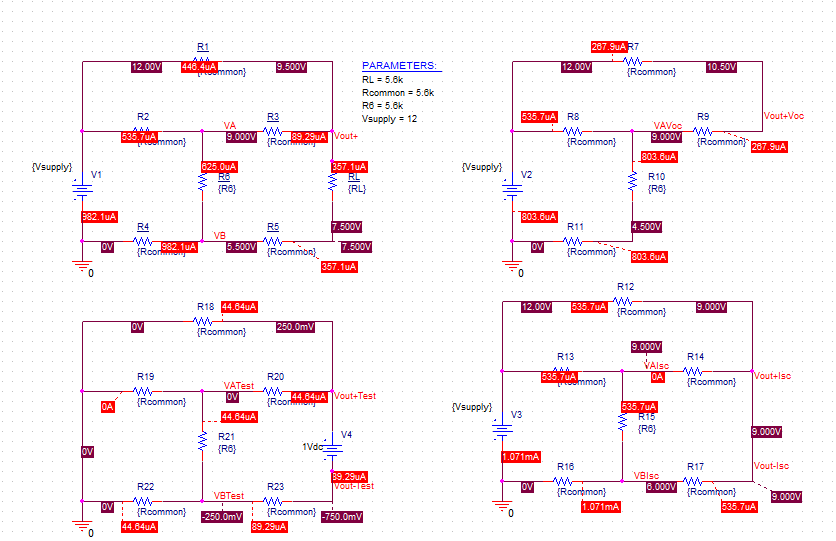
\includegraphics[width=\textwidth]{schematic_1}
		\caption{Screen shot of the PSPICE schematic with voltage markers.}
		\label{Fig:SchematicVoltMarkers}
	\end{center}
\end{figure} 

%Include a brief description of the figures (which subcircuit is which-i.e., The upper right schematic diagram is the Variable Load).

The top left schematic is the full circuit. The top right shows the circuit needed to calculate the Thevenin voltage. A break can be seen where the load resistor was. The bottom left depicts a test source being added to the circuit with all of the independent power sources removed. This is used to find the equivalent resistance of the circuit. The final circuit is one were there is a short across the $R_L$ to measure the current through the point when the resistance is $0\,\si\ohm$.

\subsubsection{Theory: PSPICE Simulation Varying Load Circuit}
 In this section, include: 
 \begin{itemize}
 	\item A figure with the plot of $R_L$ vs. $v_{L}$ from PSPICE.
 	\item A figure with the corresponding linear regression in Excel that illustrates the resulting scatter plot and extraction of $R_{th}$. 
 	\item Present the equation generated by Excel in the text of the report.
 	\item Be sure to indicate the $r^2$  value with the equation. You may need to change the output precision of Excel if the $r^2$ value appears to be ``1''.  Realistically simulation results will show a ``1''.
 	\item Table \ref{Table:Lab3VariableLoadPSPICE} shows the Thevenin voltage and resistance calculated from the excel document. The results agree with that of the tutorial.
 	\begin{table}[h]
 		\centering
 		\caption{Variable Load PSPICE test results}.
 		\label{Table:Lab3VariableLoadPSPICE}
 		%\begin{tabular}{llllll}
 		\begin{tabular}{|c|c|c|c|}
 			\hline
 			$V_{th}$ (\si{\volt})& %$I_{sc}$ (\si{\milli\ampere}) &
 			 $R_{th}$ (\si{\ohm}) \\
 			\hline
 			10.629	& 2514.3 \\	 \hline 
 		\end{tabular}
 	\end{table}
 \end{itemize}
 
\subsubsection{Theory: PSPICE Simulation Open Circuit/Short Circuit Test}
 In this section, include: 
 \begin{itemize}
 	\item Explain how the PSPICE schematic was altered for the open circuit voltage test and short circuit test. The entire discussion (including all bullets below) should be about 1 paragraph
 	\item Refer to the Fig. \ref{Fig:SchematicVoltMarkers} with a screen shot of the schematic in PSPICE with voltage markers for the $V_{oc}$ test.  As you likely have already placed this figure in your theory section, there is no need to do so a second time.  
 	\item Refer to Fig. \ref{Fig:SchematicCurrentMarkers} with a screen shot of the schematic in PSPICE with current markers for the $I_{sc}$ test.  As you likely have already placed this figure in your theory section, there is no need to do so a second time.  

 	 \begin{table}[h!]
 	 	\centering
 	 	\caption{PSPICE Open/Short Test Table}.
 	 	\label{Table:Lab3VocIscPSPICE}
 	 	%\begin{tabular}{llllll}
 	 	\begin{tabular}{|c|c|c|c|}
 	 		\hline
 	 		$V_{th}$ (\si{\volt})& $I_{sc}$ (\si{\milli\ampere}) & $R_{th}$ (\si{\ohm}) \\
 	 		\hline
 	 		10.629 & 0.004227 & 2.515.022 \\	 \hline 
 	 	\end{tabular}
 	 \end{table}
 \end{itemize}
 
Table \ref{Table:Lab3VocIscPSPICE} shows the $R_{th}$ calculations when the voltage across the load is measured with a break and the current through the load is measured with a short. The results agree with the PSPICE simulation.
 
\subsubsection{Theory: PSPICE Simulation Test Signal Method }
 In this section, include: 
 \begin{itemize}
 	\item Explain how the PSPICE schematic was altered for the open circuit voltage test and short circuit test. The entire discussion (including all bullets below) should be about 1 paragraph
 	\item Refer to the Fig. \ref{Fig:SchematicCurrentMarkers} with a screen shot of the schematic in PSPICE with current markers for the Test signal.  As you likely have already placed this figure in your theory section, there is no need to do so a second time.  
 	
 
 	\item The results in Table \ref{Table:Lab3ReqTestSignalPSPICE} agree with the results from $V_{OC}$ and $I_{SC}$ in the tables about. This table shows the thevenin resulting circuit if a 1V source was added. 
 		\begin{table}[h!]
 			\centering
 			\caption{$R_{th}$ from Test Signal.}
 			\label{Table:Lab3ReqTestSignalPSPICE}
 			%\begin{tabular}{llllll}
 			\begin{tabular}{|c|c|c|c|c|c|}
 				\hline
 				Test Signal  (\si{\volt}) &$V_{R5}$ (\si{\volt}) & $I_{\mbox{Test Signal}}$ (\si{\milli\ampere}) & $R_{th}$ (\si{\ohm})\\
 				\hline
 				1 & .3977 & 0.0003977 & 2514k \\	 \hline 
 			\end{tabular}
 		\end{table}
 \end{itemize}

\section{Hardware Experiment: Results and Discussion}
This section of the report should present what was done in hardware.  A reader should be able to recreate an experiment from the detail present.  One section discusses the equipment used in the experiment. The remaining sections discuss the results for each circuit.
\subsection{Equipment Used in the Laboratory}
Write a short paragraph to detail the equipment used in the laboratory, and specific model numbers. Ideally, you should create a table of the equipment which should be referred to in text (See Table \ref{Table:Equipment} as an example).  The room location where the experiment was performed should be included.  Note that this should be a part of all Tech Memos, as it is an essential piece for other users to replicate your experiment.  \textbf{As you will be likely using the same equipment throughout the term, once the text/tables are established, you may reuse the information with the permission of your instructor/TA. Again, cite your first lab report as a reference.}
		
		\begin{table}[h!]
			\centering
			\caption{Equipment/Software required for Lab 2.}
			\label{Table:Equipment}
			%\begin{tabular}{llllll}
			\begin{tabular}{|c||c|c|c|c|}
				\hline
				Item & Tool & Room      \\
				\hline
				Simulation & OrCAD Capture CIS & All Open EE Labs   \\	 
				\hline 
				DC Power Supply&  Agilent E3630A  & 09-3170   \\	
				\hline  
				DC Power Supply & Agilent E3631A   & 09-3200 \\ 
				\hline 
				Multimeter & Agilent E34401A   & 09-3170, 09-3200 \\ 
				\hline 
			%	Waveform Generator & Agilent 33120A & 09-3170, 09-3200 \\
			%	\hline
			%	Oscilloscope & Textronix TDS2012C & 09-3200  \\
			%	\hline
			%	Oscilloscope & Agilent DSO 33120A & 09-3170  \\
			%	\hline
			\end{tabular}
		\end{table}
\subsection{Hardware Results/Discsussion Resistor Values}	
  Begin the section by including the experimental values of the resistors as illustrated in Table \ref{Table:Lab3Resistors}. If you kept your lab 2 circuit wired up for lab 3, you can include the table (cut/paste), citing your lab 2 report. Briefly discuss.
  	\begin{table}[h!]
  		\centering
  		\caption{Resistors used in the laboratory.}
  		\label{Table:Lab3Resistors}
  		%\begin{tabular}{llllll}
  		\begin{tabular}{|c||c|c|c|c|}
  			\hline
  			Resistor &Exp. Value (\si{\kilo\ohm})  \\
  			\hline
  			$R_{1}$  &   \\	 \hline 
  			$R_{2}$  & \\	 \hline 
  			$R_{3}$  & \\	 \hline 
  			$R_{4}$  & \\	 \hline 
  			$R_{5}$  & \\	 \hline 
  			$R_{6}$  &  \\	 \hline
  		\end{tabular}
  	\end{table}
  \subsection{Hardware Results: Open/Short Extraction}
  
  \begin{table}[h!]
  	\centering
  	\caption{Hardware Open/Short Test Table}.
  	\label{Table:Lab3VocIsc}
  	%\begin{tabular}{llllll}
  	\begin{tabular}{|c|c|c|c|}
  		\hline
  		$V_{th}$ (\si{\volt})& $I_{sc}$ (\si{\milli\ampere}) & $R_{th}$ (\si{\ohm}) \\
  		\hline
  		& &  \\	 \hline 
  	\end{tabular}
  \end{table}
  Include the following discussion points in a paragraph:
  \begin{itemize}
  	\item A table of the measured open circuit voltage and short circuit current  (Table \ref{Table:Lab3VocIsc}).
  	\item Provide a discussion of how you implemented the technique in hardware (i.e., What did you change in the hardware circuit to measure the open circuit voltage?  What did you change in the hardware circuit to measure the short circuit current?)
  	\item For the short circuit current, you most likely extracted this by measuring a voltage across the $R_5$ resistor in the lab handout.  Include the Ohm's law calculation to back out the current as an inline equation. 
  	\item Discuss how the results agree with theory, and include an error analysis based on either the PSPICE or hand calculations.
  \end{itemize}
  \subsection{Hardware Results: Direct Measurement of $R_{th}$}
  In this section, discuss the  direct measurement of $R_{th}$ in  1 paragraph.
  \begin{itemize}
  	\item Provide a discussion of how you implemented the technique in hardware.  What was done to the load resistor? What was done to the power supply?  How was $R_{th}$ measured?
  	\item Record the value of $R_{th}$ from direct measurement in Table \ref{Table:Lab3RthDirect}.
  	\item Discuss whether the results agree with theory.
  \end{itemize}
  \begin{table}[h!]
  	\centering
  	\caption{$R_{th}$ direct measurement table}
  	\label{Table:Lab3RthDirect}
  	%\begin{tabular}{llllll}
  	\begin{tabular}{|c|c|c|c|}
  		\hline
  		$R_{th}$ (\si{\kilo\ohm})&\hspace{2in} \\
  		\hline 
  	\end{tabular}
  \end{table}
  \subsection{Hardware Results:  Test Signal Extraction}
  In this section, discuss the  test signal extraction measurement of $R_{th}$ in  1 paragraph.
  \begin{itemize}
  	\item Provide a discussion of how you implemented the technique in hardware.  What was done to the load resistor? What was done to the power supply? Where did you hook up the test signal, and what was the magnitude of the test signal? How was $R_{th}$ determined?
  	\item Record the value of $R_{th}$ from the test signal extraction in Table \ref{Table:Lab3ReqTestSignal}.
  	\item Discuss whether the results agree with theory.
  	\item Answer the following question: If the test signal was increase to 3~\si{\volt}, would the final result change? Explain.
  \end{itemize}
  \begin{table}[h!]
  	\centering
  	\caption{$R_{th}$ from Test Signal.}
  	\label{Table:Lab3ReqTestSignal}
  	%\begin{tabular}{llllll}
  	\begin{tabular}{|c|c|c|c|c|c|}
  		\hline
  		Test Signal  (\si{\volt}) &$V_{R5}$ (\si{\volt}) & $I_{R5}=i_{test}$ (\si{\milli\ampere}) & $R_{th}$ (\si{\ohm})\\
  		\hline
  		& & &  \\	 \hline 
  	\end{tabular}
  \end{table}
  
  \subsection{Hardware Results: Varying Load Extraction}
  In this section, you should discuss the hardware results of the varying load extraction.  Include the following:
  \begin{itemize}
  	\item A table of the measured load voltage, and corresponding load current for each resistor (Table \ref{Table:Lab3LoadResistors}).
  	\item A scatter plot of this data  in Excel/Matlab/etc. showing the line fit extraction and corresponding Th\'evenin Resistance.   As described in the prelab video, be sure to indicate the $r^2$  value with the equation. You may need to change the output precision of Excel if the $r^2$ value appears to be ``1''. 
  	\item Briefly discuss whether the results compare to the PSPICE theory.
  \end{itemize}
  	\begin{table}[h!]
  		\centering
  		\caption{Variable load resistor Table.  Use Ohm's Law to determine the load current ($I_L$)}.
  		\label{Table:Lab3LoadResistors}
  		%\begin{tabular}{llllll}
  		\begin{tabular}{|c||c|c|c|c|}
  			\hline
  			Resistor &Exp. Value (\si{\kilo\ohm}) &$V_{RL}$ (\si{\volt}) & $I_L$ (\si{\ampere}) \\
  			\hline
  			$R_{L1}$  & & & \\	 \hline 
  			$R_{L2}$  & & & \\	 \hline 
  			$R_{L3}$  & & & \\	 \hline 
  			$R_{L4}$  & & & \\	 \hline 
  			$R_{L5}$  & & & \\	 \hline 
  			$R_{L6}$  & & & \\	 \hline
  			$R_{L7}$  & & & \\	 \hline
  			$R_{L8}$  & & & \\	 \hline 
  		\end{tabular}
  	\end{table}
 
	\section{Conclusion}
	Provide a 1 paragraph summary of the laboratory experiment.  What were the major conclusions for each part of the experiment?  Also did the theory agree with the experiment?  The conclusion is a revised version of the abstract.  Has Th\'evenin's Theorem been experimentally validated?  Discuss the effects of tolerances affecting the differences between measured results and simulated results.
	\section{Acknowledgments}
	Acknowledge \textbf{any} source of help received in the experiment/writing the report.  This should certainly include your lab partner/teaching assistant/instructor.  It may also include other classmates/study partners. State briefly what the nature of the help was.
	
	\textbf{Your report should include references to appropriate pages in the text, as well as any other sources, websites/etc. consulted in the preparation of the report.}
\begin{thebibliography}{9}
	\bibitem{AlexanderSadiku}
	C.K. Alexander, and M.K.O. Sadiku,
	\emph{Fundamentals of Electric Circuits, 4th Edition},
	McGraw Hill, pp. xx-yy(EDIT), 2009.
	\bibitem{OldLab}
A. Student,
	\emph{EEEE 281 Lab 1 Tech Memo},
	page xx-yy, submitted Month, Day, 2015.
	\bibitem{RommelLab}
	S. Rommel,
	\emph{EEEE 281 Lab 1 Lecture notes},
	slides xx-yy, Spring 2015.
\end{thebibliography}

\end{document}



